\documentclass[12pt]{article}
\usepackage[utf8]{inputenc}
\usepackage{graphicx} % Allows you to insert figures
\usepackage{amsmath} % Allows you to do equations
\usepackage{fancyhdr} % Formats the header
\usepackage{geometry} % Formats the paper size, orientation, and margins
\linespread{1.25} % about 1.5 spacing in Word
\setlength{\parindent}{0pt} % no paragraph indents
\setlength{\parskip}{1em} % paragraphs separated by one line
\usepackage[format=plain,
            font=it]{caption} % Italicizes figure captions
\usepackage[english]{babel}
\usepackage{csquotes}
\renewcommand{\headrulewidth}{0pt}
\geometry{letterpaper, portrait, margin=1in}
\setlength{\headheight}{14.49998pt}

\newcommand\titleofdoc{\textbf{Assignment-5: Laplace Equation}}
\newcommand\GroupName{EE20B136}

\begin{document}
\begin{titlepage}
   \begin{center}
        \vspace*{4cm} % Adjust spacings to ensure the title page is generally filled with text

        \Huge{\titleofdoc} 

        \vspace{3 cm}
        \Large{Syam SriBalaji T}
       
        \vspace{0.25cm}
        \large{EE20B136}
       
        \vspace{3 cm}
        \Large{March 11, 2022}
        
        \vspace{0.25 cm}
        \Large{EE2703 :Jan-May 2022}
       

       \vfill
    \end{center}
\end{titlepage}

\setcounter{page}{2}
\pagestyle{fancy}
\fancyhf{}
\rhead{\thepage}

\section*{Initial Potential configuration}

Here we can see Initial Potential contour plot, where yellow region specifies 1V and red region specifies 0V\\
Also here we can view the approximation of circle for the given values done in this plate.\\

\begin{figure}[h!]
\centering
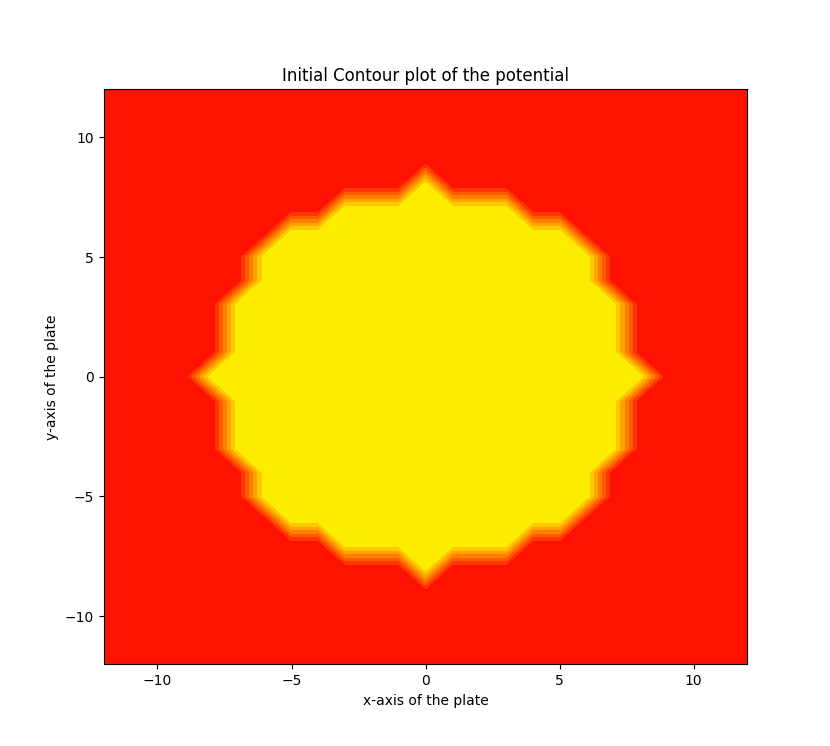
\includegraphics[height=14cm]{Figure_1.png}
\end{figure}

\newpage
\section*{Plot for Error vs. Number of Iteration}

For finding error, we find new potentials for each iteration using Vectorization method and subtract the new ones from the old ones.\\
Here we can clearly see that, as the number of Iteration increases the error decreases because as we know more the number of Iteration gives precise potential values.\\

\begin{figure}[h!]
\centering
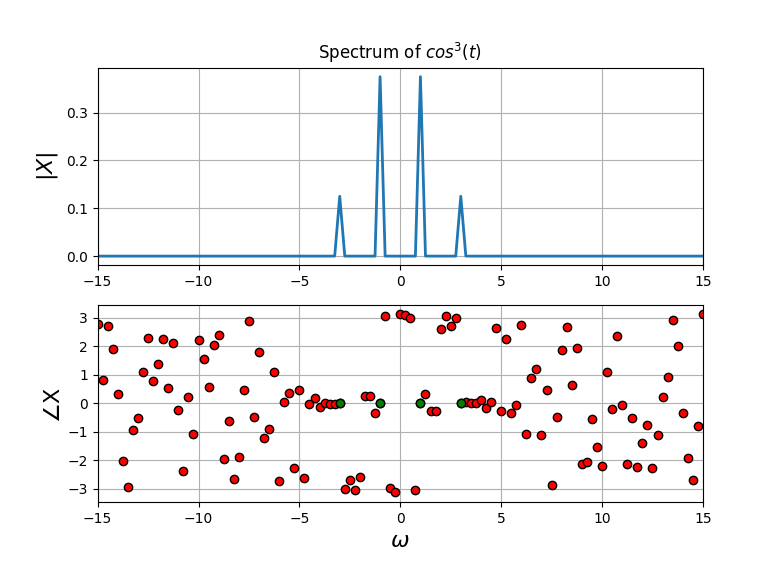
\includegraphics[height=14cm]{Figure_2.png}
\end{figure}

\newpage
\section*{Semilog plot for Error vs. Number of Iteration}

Same above plot is drawn in Semilog graph here, and we can observe change in slope at a particular point. And as number of Iteration increases, Error varies linearly with negative slope.\\

\begin{figure}[h!]
\centering
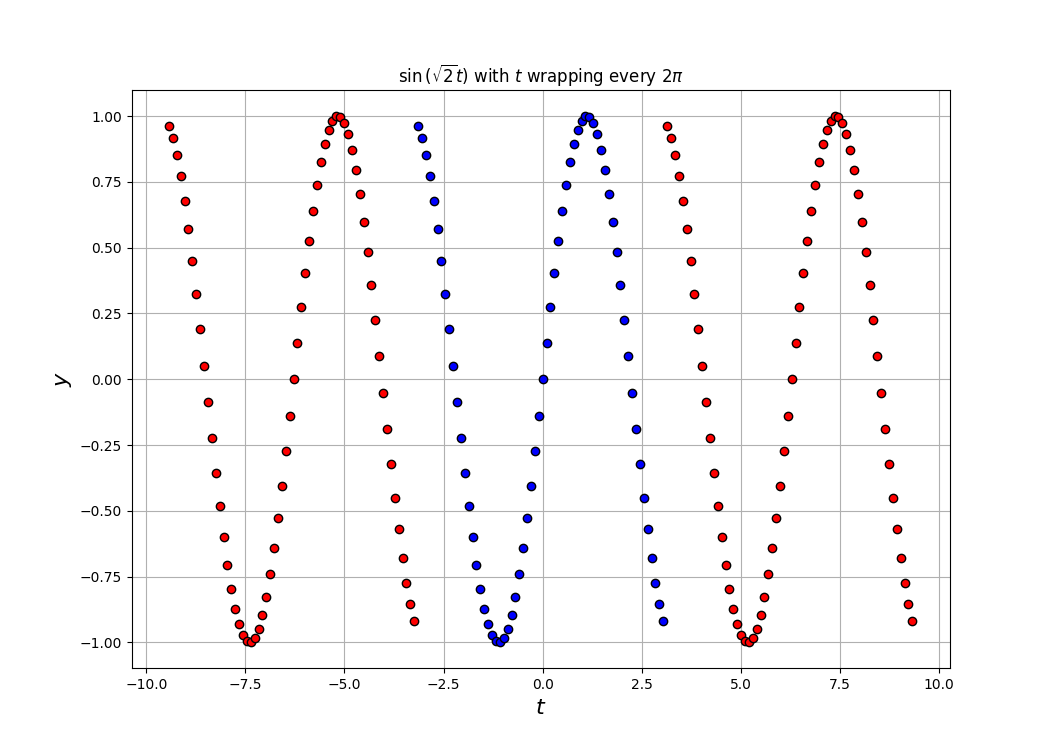
\includegraphics[height=14cm]{Figure_3.png}
\label{fig:exemplo}
\end{figure}

\newpage
\section*{Loglog plot for Error vs. Number of Iteration}

Same above plot is drawn in Loglog graph here, and we can see that Error varies exponentially with respect to number of Iteration.\\

\begin{figure}[h!]
\centering
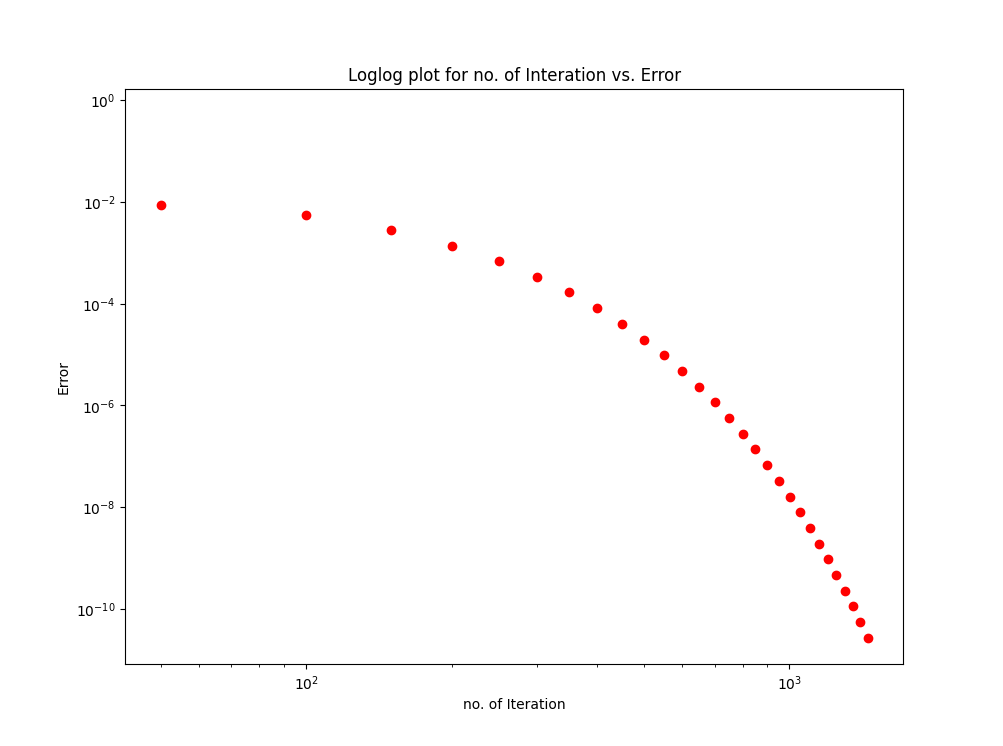
\includegraphics[height=14cm]{Figure_4.png}
\label{fig:exemplo}
\end{figure}

\newpage
\section*{Comparison of plots found from different methods}

Here,\\ Fit-1: Error plot from Vectorization method \\ Fit-2: Error plot from lstsq method (error minimization)\\\\
So, we can clearly see that both of the graph coincide. Also we can see very little deviation in values where Number of iteration is less and rest coincides perfectly where Number of iteration is more.\\


\begin{figure}[h!]
\centering
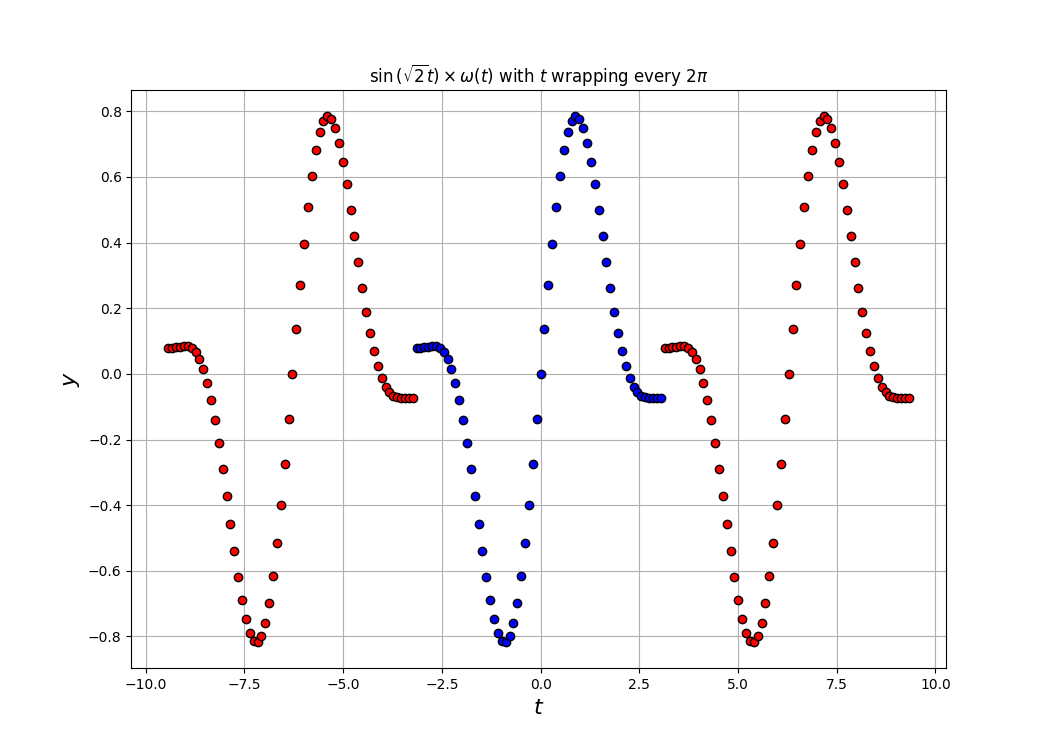
\includegraphics[height=14cm]{Figure_5.png}
\label{fig:exemplo}
\end{figure}

\newpage
\section*{Plotting Cumulative error graph with Stopping condition}

As given from derivation in assignment, Error with Stopping condition = $-\dfrac{A}{B} $e^{(B(N+0.5))}$ \\\\
From this formula, we find error for each number of Iteration, and then using that we find cumulative error graph. And we can see that it is increasing with increase in number of iteration as shown below, and as the number of iteration becomes very more, this almost becomes parallel.\\

\begin{figure}[h!]
\centering
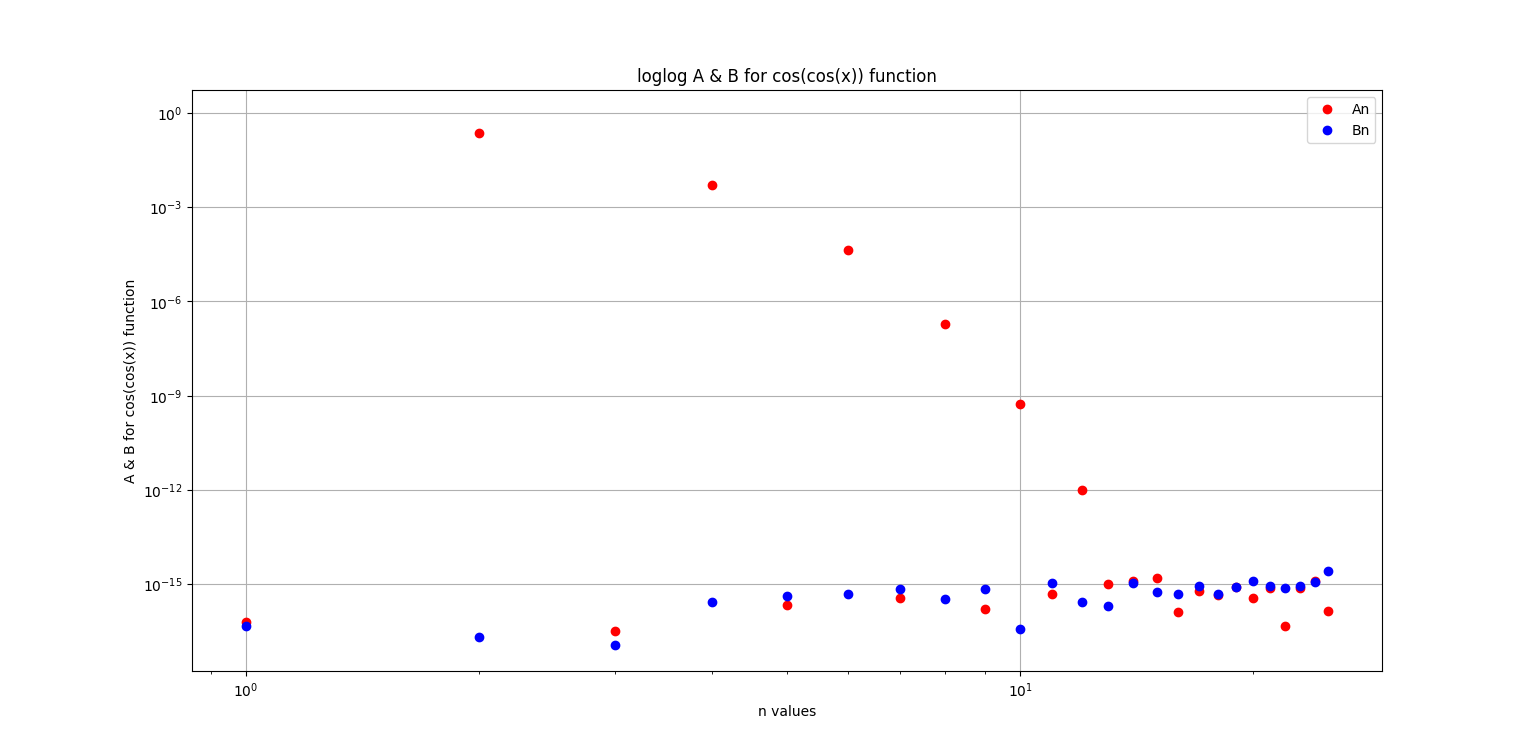
\includegraphics[height=14cm]{Figure_6.png}
\label{fig:exemplo}
\end{figure}

\newpage
\section*{3-D Surface Plot of Potential}

Here we can 3-D Surface plot of potential, In this plot we can clearly note that the top part of the plate is having 1 V, middle part having 1 V and bottom part of the plate is having  0 V.\\

\begin{figure}[h!]
\centering
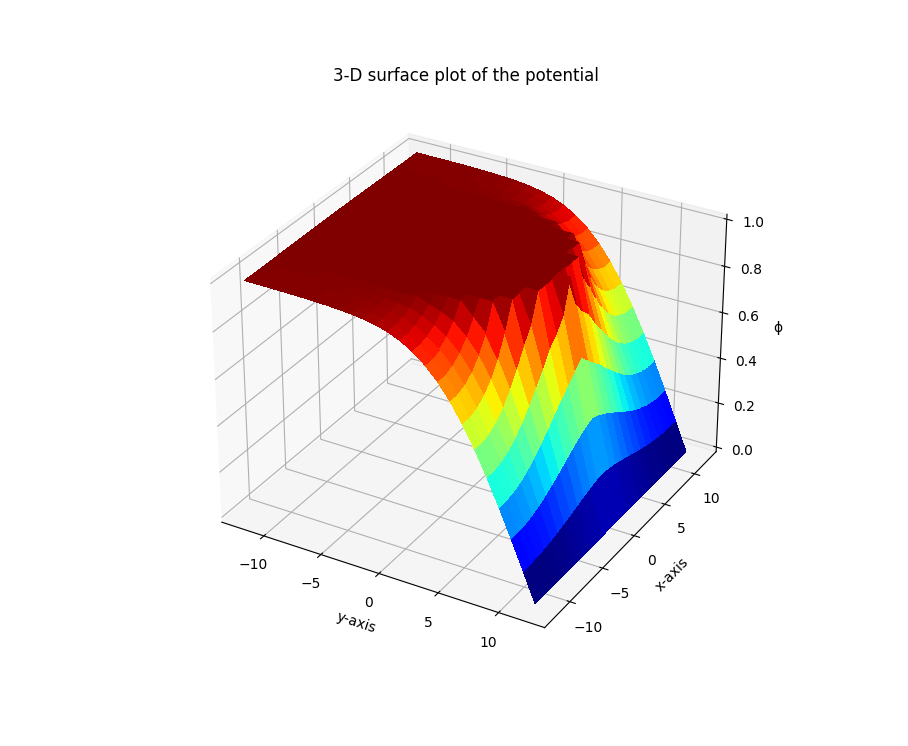
\includegraphics[height=17cm]{Figure_7.png}
\label{fig:exemplo}
\end{figure}

\newpage
\section*{Contour Plot of the Potential}

Here, we can see Contour plot of potential and range of magnitude of potential can be found from the bar near it.\\

\begin{figure}[h!]
\centering
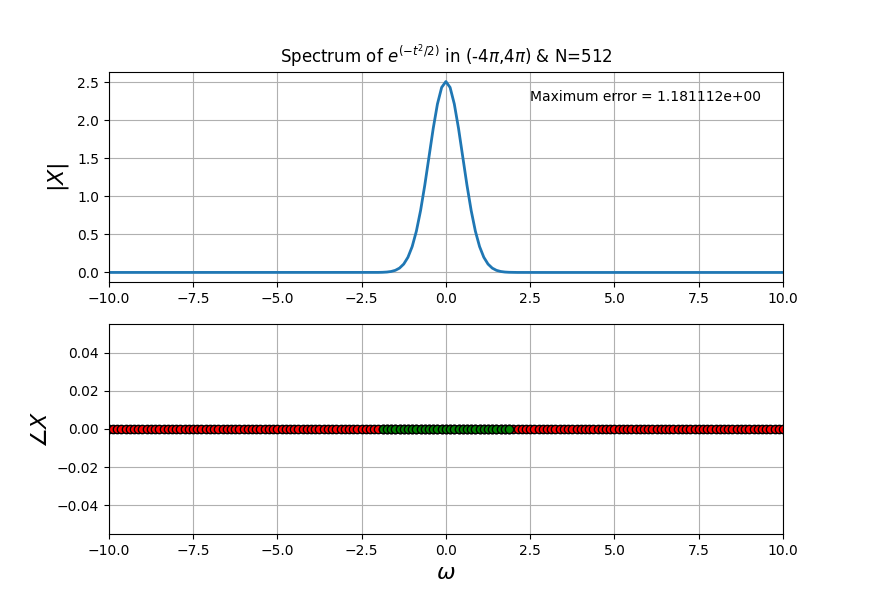
\includegraphics[height=14cm]{Figure_8.png}
\label{fig:exemplo}
\end{figure}


\newpage
\section*{Vector plot of the current flow}

From the derivation and formula given in assignment, we plot the 2-D plot of  Current density vector and we can clearly see current moving from high voltage to low voltage (top to bottom).\\

\begin{figure}[h!]
\centering
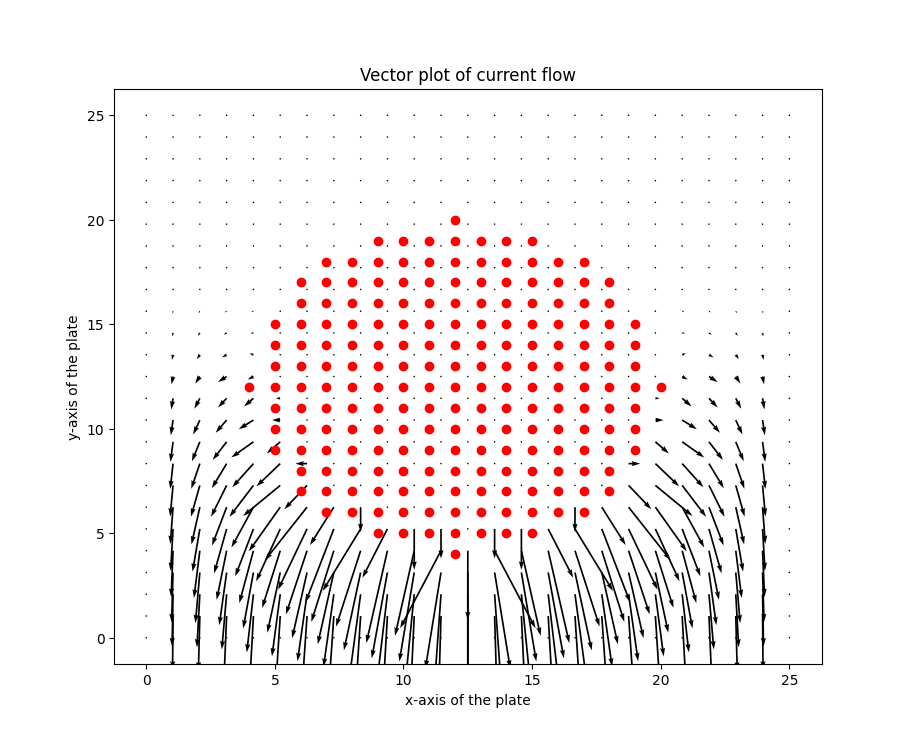
\includegraphics[height=14cm]{Figure_9.png}
\label{fig:exemplo}
\end{figure}

\begin{center} 
\textbf{Thank you!}
\end{center} 
\end{document}
